\section{Differenze di implementazione}\label{sec:ddimpl}


\subsection{Database}

Rispetto al modello iniziale del database, sono state effettuate alcune
piccole modifiche riguardanti la sua struttura interna. Queste modifiche
sono state necessarie in quanto il framework utilizzato \textbf{EJP}
(\emph{Easy Java Persistence}) ``obbliga'' ad esempio,  la strutturazione della 
progettazione delle classi del database.
Tuttavia le piccole modifiche applicate sono compensate da una potenza
di espressione e semplicità di utilizzo dello stesso per raggiungere
gli obbiettivi prefissati.

In seguito ad alcuni problemi riscontrati nello stesso framework,
sono state rimosse tutte le referenze dal database e, per semplificare
ulteriormente il mapping delle classi all'interno del database, sono
stati modificati alcuni campi nelle singole relazioni.

\lstinputlisting[language=SQL]{database/DATABASE2.sql}

\subsection{Amministratore}

Come stabilito con il cliente, esistono due amministratori predefiniti
all'interno del sistema; siccome questi devono esistere sempre abbiamo
deciso di creare due amministratori che vengono automaticamente inseriti
all'interno del database durante la creazione dello stesso. Gli amministratori
si distinguono come:
\begin{itemize}
\item Reparto di Ortopedia

\begin{itemize}
\item username:\emph{ }\textbf{\emph{admino}}
\item password: \textbf{\emph{admino}}
\end{itemize}
\item Reparto di Pediatria

\begin{itemize}
\item username: \textbf{\emph{adminp}}
\item password:\emph{ }\textbf{\emph{adminp}}
\end{itemize}
\end{itemize}
Questi possono essere cambiati semplicemente effettuando un query
al database (dall'amministratore del database), oppure l'amministratore
può cambiare i propri dati di accesso da interfaccia grafica.


\subsection{Modifica del modello di business}
\begin{figure}[!thp]
	\centering
	\subfloat[][\emph{Package diagram for the whole project}.]{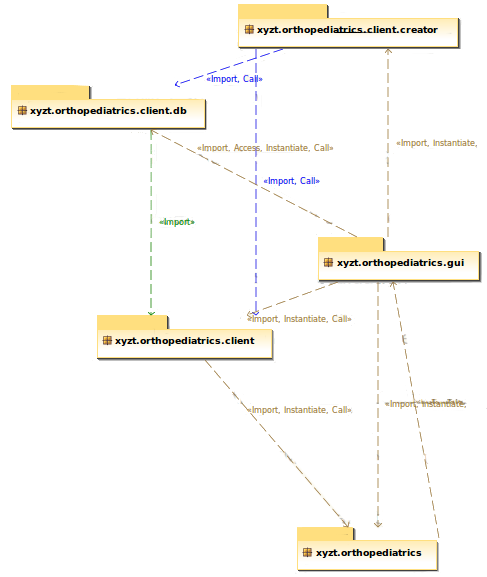
\includegraphics[scale=0.6]{lastdiagrs/package}}\\
	\subfloat[][\emph{New organization for Database Data Management}.]{\label{subfig:database}
\includegraphics[scale=0.6]{lastdiagrs/database}}\\
	\caption{\it{Implementation's View (1)}.}
	\label{fig:implviewone}
\end{figure}
Rispetto al modello iniziale di progettazione delle classi, sono state
effettuate alcune modifiche semplificando ulteriormente la struttura
interna delle classi; queste modifiche (come detto in precedenza)
sono una conseguenza dovuta in parte all'impiego del framework \textbf{\emph{EJP}},
e in parte ad una scelta di progettazione, in quanto vengono divise
le singole responsabilità delle classi. In dettaglio è voluto spostare
le funzionalità contenute all'interno delle classi del modello di
dominio (in particolare Paziente, Amministratore e Tutore) nelle classi
\emph{``Creator}'' che caratterizzano il design pattern ``\emph{Abstract
Factory}'' (v. Figura \vref{fig:implviewone}\subref{subfig:database}).

\begin{figure}[!thp]
	\centering
	\subfloat[][\emph{Classes used for direct Database mapping}.]{\label{subfig:dmapping}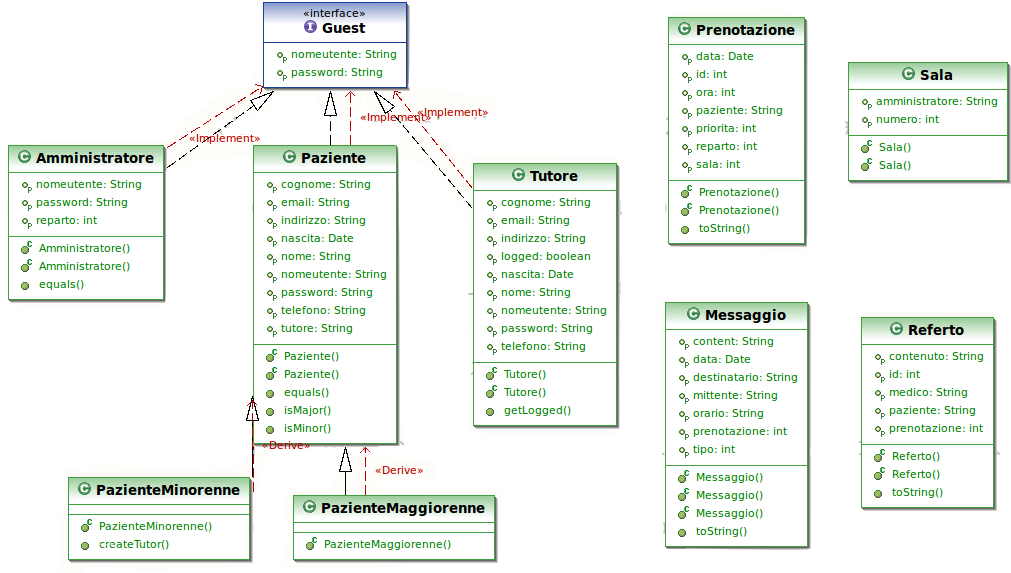
\includegraphics[scale=0.5]{lastdiagrs/client_package}}\\
	\subfloat[][\emph{Database Mapping and GUI strate}.]{\label{subfig:dmapandGUI}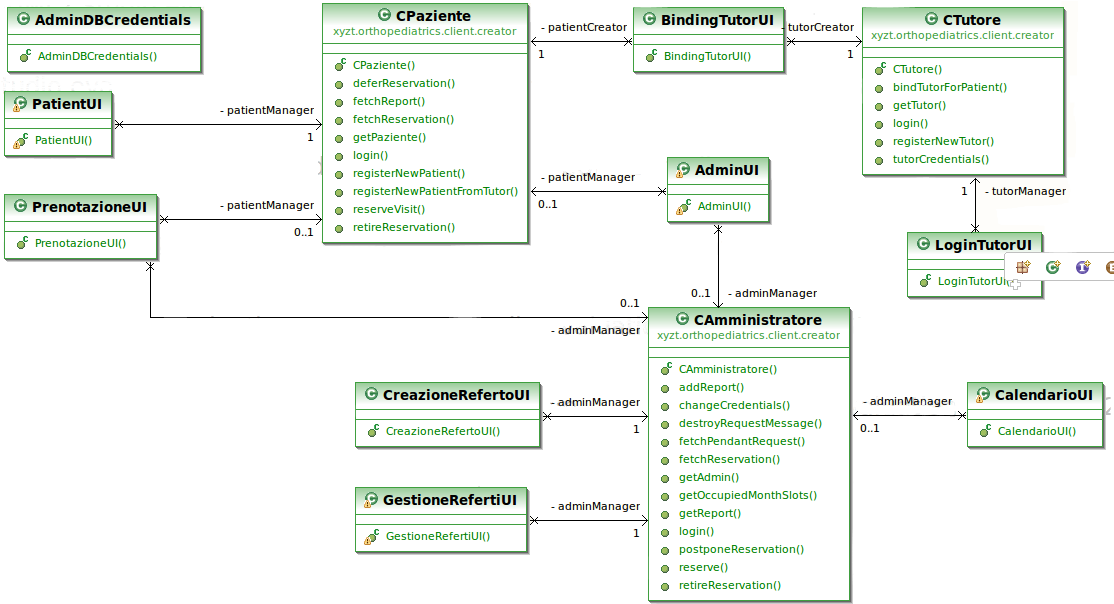
\includegraphics[scale=0.45]{lastdiagrs/usingMagagers}}\\
	\caption{\it{Implementation's View (1)}.}
	\label{fig:implviewtwo}
\end{figure}
Inizialmente la gestione dei messaggi era di responsabilità di due
classi distinte: \emph{MAmministratore} e \emph{MPaziente}, contenenti
rispettivamente i messaggi diretti all'amministratore e al paziente.
Si è voluto unificare tale modello in un unica classe \textbf{Messaggio}
contenete i messaggi diretti ad entrambi gli utenti del sistema (Amministratore
e Paziente), distinguendoli come \emph{mittente} e \emph{destinatario} (v.
Figura \vref{fig:implviewtwo}\subref{subfig:dmapping}). Possiamo inoltre
evidenziare tramite la Figura \vref{fig:implviewtwo}\subref{subfig:dmapandGUI}
come sia stata realizzata l'interazione tra database ed interfaccia grafica,
senza la necessità di ricorrere all'implementazione di uno strato intermedio.

\begin{figure}[!thp]
	\centering
	\subfloat[][\emph{Loading admin's Message Request list}.]{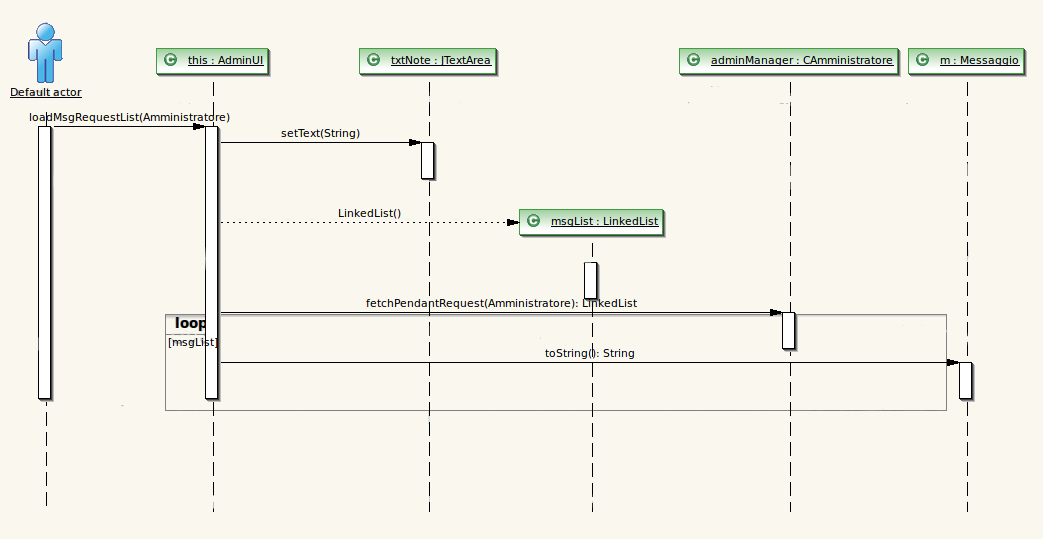
\includegraphics[scale=0.5]{lastdiagrs/admin_load_msg_req_list}}\\
	\subfloat[][\emph{Getting current Ward's prenotations}.]{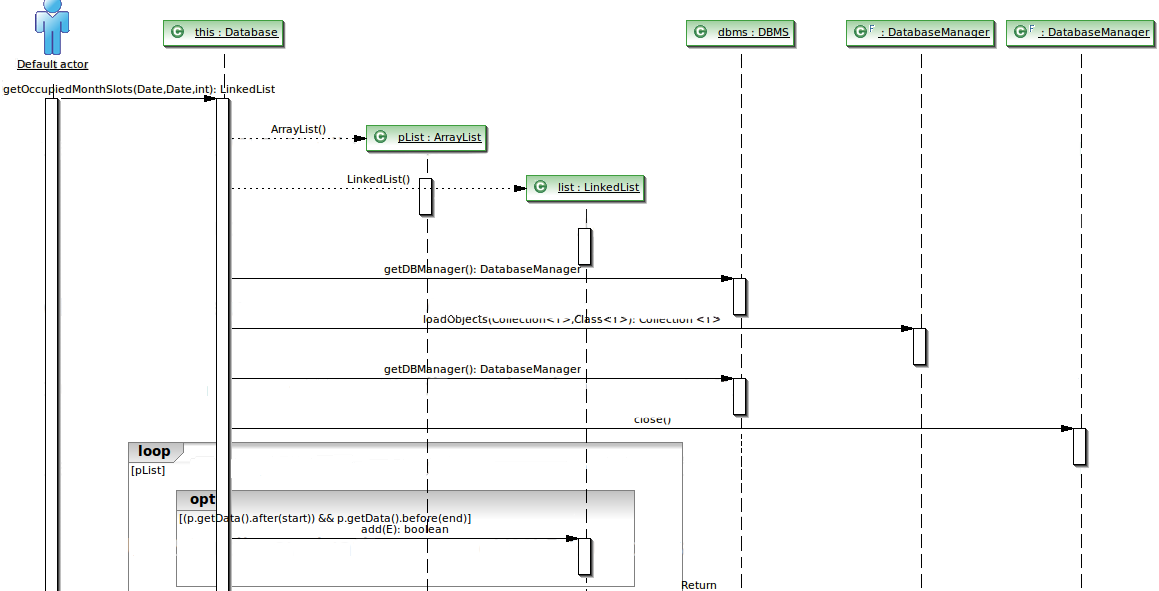
\includegraphics[scale=0.45]{lastdiagrs/getoccupiedmonthslots}}\\
	\caption{\it{Some interaction diagrams for the final implementation}.}
	\label{fig:implviewtre}
\end{figure}[!thp]
\begin{figure}
\centering
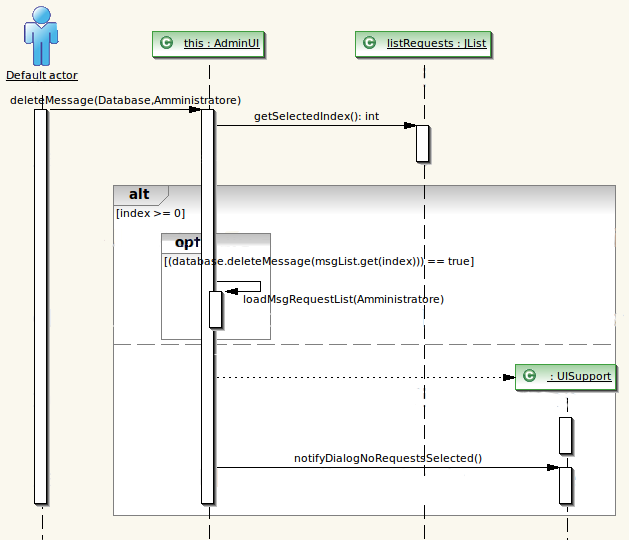
\includegraphics[scale=0.5]{lastdiagrs/admin_ui_delete_message}
\caption{\textit{Deleting received Request Messages}.}
\label{fig:implviewfou}
\end{figure}
Possiamo inoltre evidenziare tramite i diagrammi rappresentati in Figura
\vref{fig:implviewtre} e \vref{fig:implviewfou}, come questi possano differire 
rispetto a quelli presentati nella Sottosezione \vref{subsec:projagliobj}.
